\chapter{RESULTADOS NUMÉRICOS}\label{sec:resultados}

%\begin{itemize}
%	\item \textcolor{red}{IGOR: já fiz uma primeira revisão deste capítulo e indico em vermelho o que deve fazer para melhorar este capítulo. Tudo que acrescentar ou mudar coloque em azul.} \textcolor{green}{OK}
%	\item \textcolor{red}{IGOR: não está aparecendo a numeração das Figuras no caption. Algo de errado está acontecendo no modelo que está utilizando.} \textcolor{green}{OK}
%	\item \textcolor{red}{IGOR: está errada a citação do trabalho do método de Duan e Zamir (1995), não é a citação que colocou \cite{Duan}.}\textcolor{green}{\textbf{OK}}
%\end{itemize}

Nesta seção, apresentam-se resultados obtidos com a implementação computacional e simulação do modelo matemático de Duan e Zamir~\cite{Duan1992}. As simulações realizadas aqui tratam da propagação de uma onda harmônica simples ao longo de uma árvore, onde reflexões de onda modificam a amplitude da onda de pressão enquanto ela avança. A escolha de uma onda harmônica simples neste estudo possibilita investigar os efeitos da frequência, fluido viscoso e viscoelasticidade da parede do segmento de vaso.

Considerou-se neste estudo um modelo de árvore arterial canina como ilustrado na Figura~\ref{fig:arvore-canina}. As propriedades dos segmentos foram escolhidas oriundas dos dados de Fung~\cite{fung2013biomechanics} e são descritas na Tabela~\ref{tab1:proprerty}. 

\begin{figure}[!htbp]
	\centering
	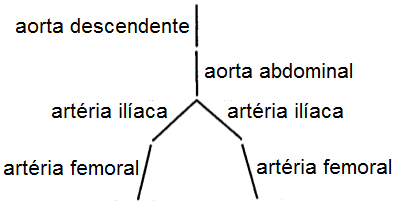
\includegraphics[scale=0.8]{Figures/tree_canine.png}
	\caption{Representação do modelo de árvore arterial canina (figura adaptada de~\cite{Duan}).}
	\label{fig:arvore-canina}
\end{figure}

\begin{table}[!htbp]
	\caption{Propriedades dos segmentos do modelo de árvore arterial~\cite{Duan,Fung}}
	\centering{}
	\begin{tabular}{c|c|c|c|c|c}
		\toprule 
		Artéria	& Comprimento & Densidade & Viscosidade  & Diâmetro & Módulo de  \\ 
		& ($cm$) & $\rho$ ($g/cm^3$) & $\mu_0$ ($g/cm s$) & ($cm$) & Young ($dyn/cm^2$) \\ 
		\midrule 
		Aorta & 25 & $0,960$ & 0,0385 & 1,3 &4,8 $\times 10^6$ \\ 
		Descendente &  & &  & & \\ 
		\hline 
		Aorta & 11 & $1,134$ & 0,0449 & 0,9 & 1,0 $\times 10^7$ \\
		Abdominal &  & &  & &  \\ 
		\hline 
		Ilíaca & 12 & $1,172$ & 0,0472 & 0,6 & 1,0 $\times 10^7$\\ 
		\hline 
		Femoral & 10 & $1,235$ & 0,0494 & 0,4 & 1,0 $\times 10^7$\\ 
		\bottomrule 
	\end{tabular} 
	\label{tab1:proprerty}
\end{table}

Nas simulações realizadas, calculou-se a distribuição de amplitude de pressão ao longo da árvore arterial (Figura~\ref{fig:arvore-canina}). Os resultados foram obtidos para quatro diferentes frequên\-cias e três diferentes cenários de escoamento/segmento: (i) escoamento viscoso em segmento puramente elástico (cenário 1 da Seção~\ref{sec:cenario}), (ii) escoamento invíscido em segmento viscoelástico (cenário 2) e (iii) escoamento viscoso em segmento viscoelástico (cenário 3). 

Os resultados obtidos nas simulações são mostrados nas Figuras~\ref{fig3a:arterial-tree}, \ref{fig3b:arterial-tree}, \ref{fig4a:arterial-tree}, \ref{fig4b:arterial-tree}, \ref{fig5a:arterial-tree} envolvendo a amplitude da pressão ao longo do modelo de árvore arterial. Nestas figuras, o comprimento de cada segmento arterial foi dimensionado para $1,0$, de modo que o comprimento adimensional total da árvore é $4,0$. O comprimento real é $58$ cm. A amplitude da pressão também foi escalada pela pressão de entrada $P_o$, e os resultados finais são portanto mostrados em termos de amplitude de pressão adimensional $|P|$ versus a distância adimensional $X$ do início da árvore.


%--------------------------------------------------------------------------------%
\section{ESCOAMENTO VISCOSO}\label{sec:cenario1}

Nas Figuras~\ref{fig3a:arterial-tree} e \ref{fig3b:arterial-tree}, o efeito da viscosidade do fluido é examinado separadamente conside\-ran\-do-se o escoamento em segmentos puramente elásticos com quatro valores diferentes de viscosidade do fluido, ou seja, $\mu = 0$; $0,5 \mu_0$; $1,0 \mu_0$ e $1,5 \mu_0$, onde $\mu_0$ é o valor base da viscosidade da Tabela~\ref{tab1:proprerty}. Observa-se que o efeito da viscosidade do fluido é reduzir o aumento global na amplitude da onda de pressão causada pelas reflexões das ondas à medida que a onda se desloca na direção à jusante. Além disso, modera os picos locais na distribuição de pressão.

\begin{figure}[!htbp]
	\centering
	(a) \\
	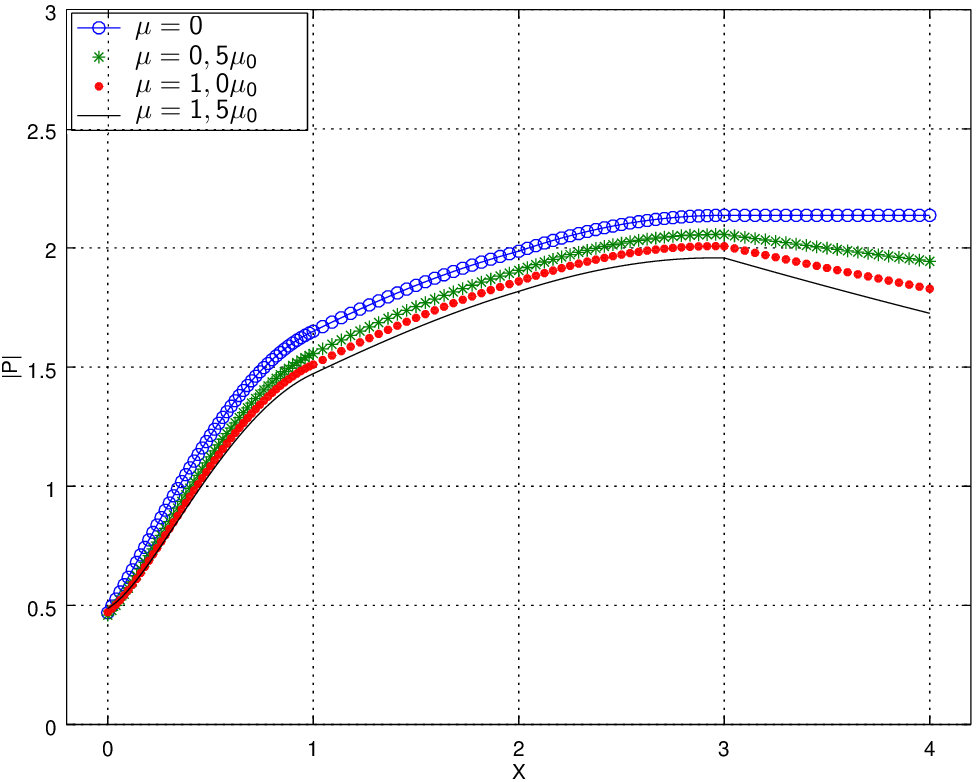
\includegraphics[scale=0.7]{Figures/fig3_P_f3_65_visc_NEW.png}\\
	(b)\\
	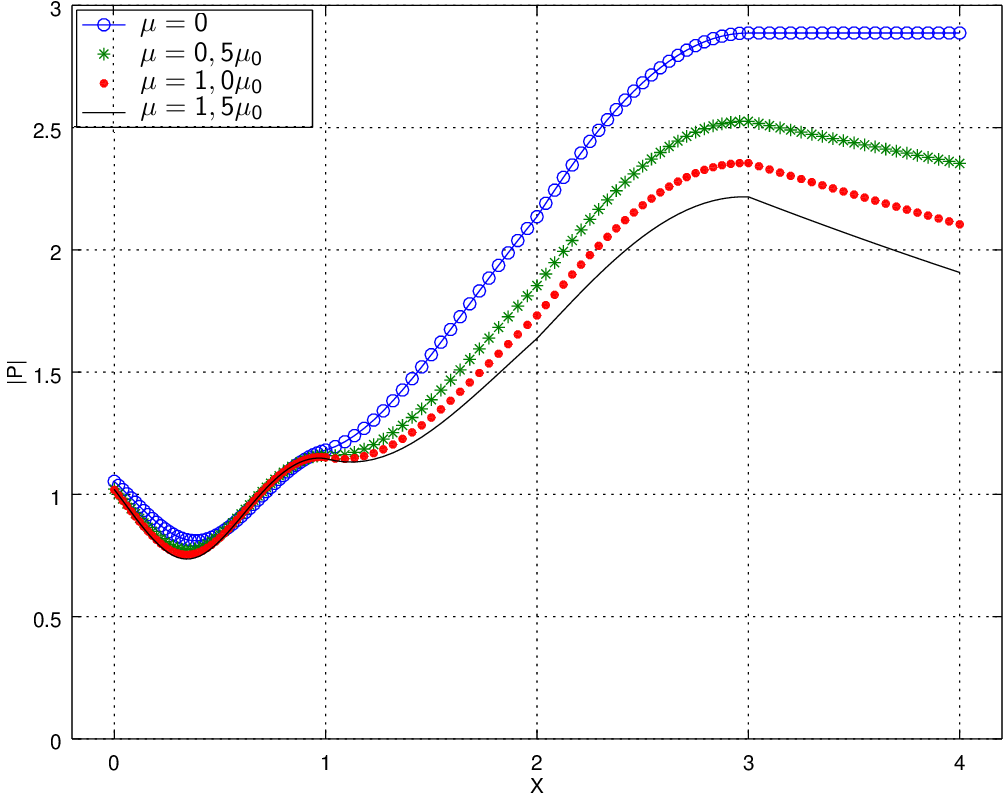
\includegraphics[scale=0.7]{Figures/fig3_P_f7_30_visc_NEW.png}\\
	\caption{Amplitude da pressão $|P|$ ao longo da árvore arterial considerando diferentes viscosidade do fluido $\mu$ e frequências: (a) $f$ = 3,65 Hz, (b)  $f$ = 7,30 Hz. }
	\label{fig3a:arterial-tree}%
\end{figure}

\begin{figure}[!htbp]
	\centering
	(a) $f$ = 10,95 Hz\\
	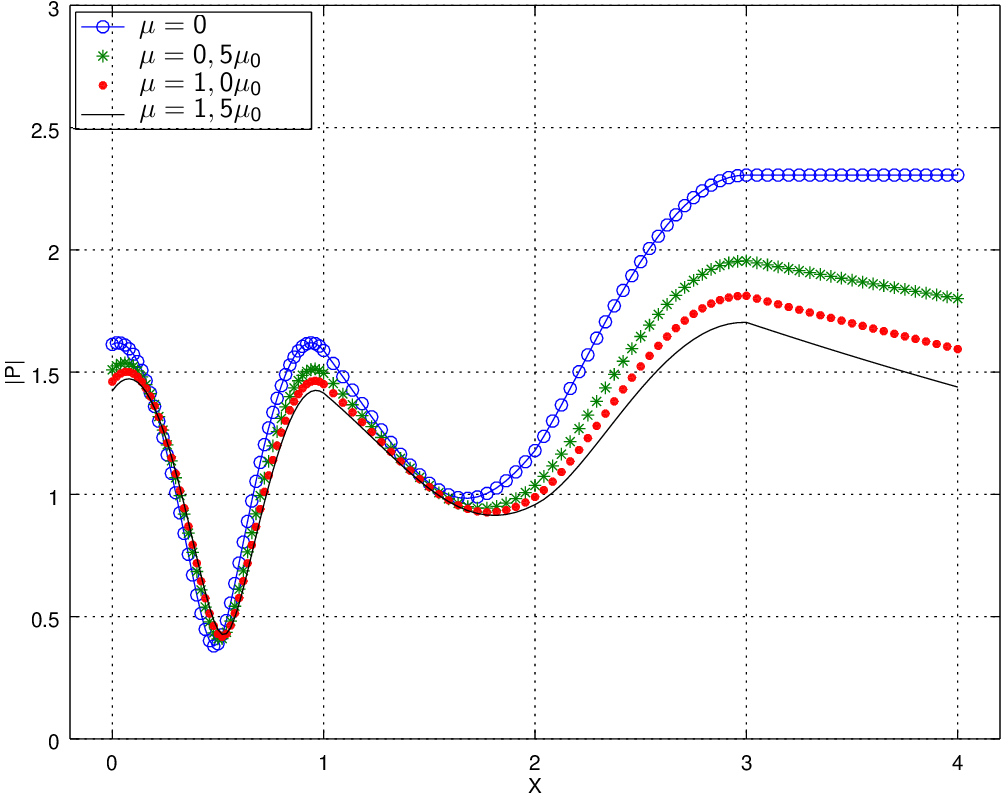
\includegraphics[scale=0.7]{Figures/fig3_P_f10_95_visc_NEW.png}\\
	(b) $f$ = 14,60 Hz\\
	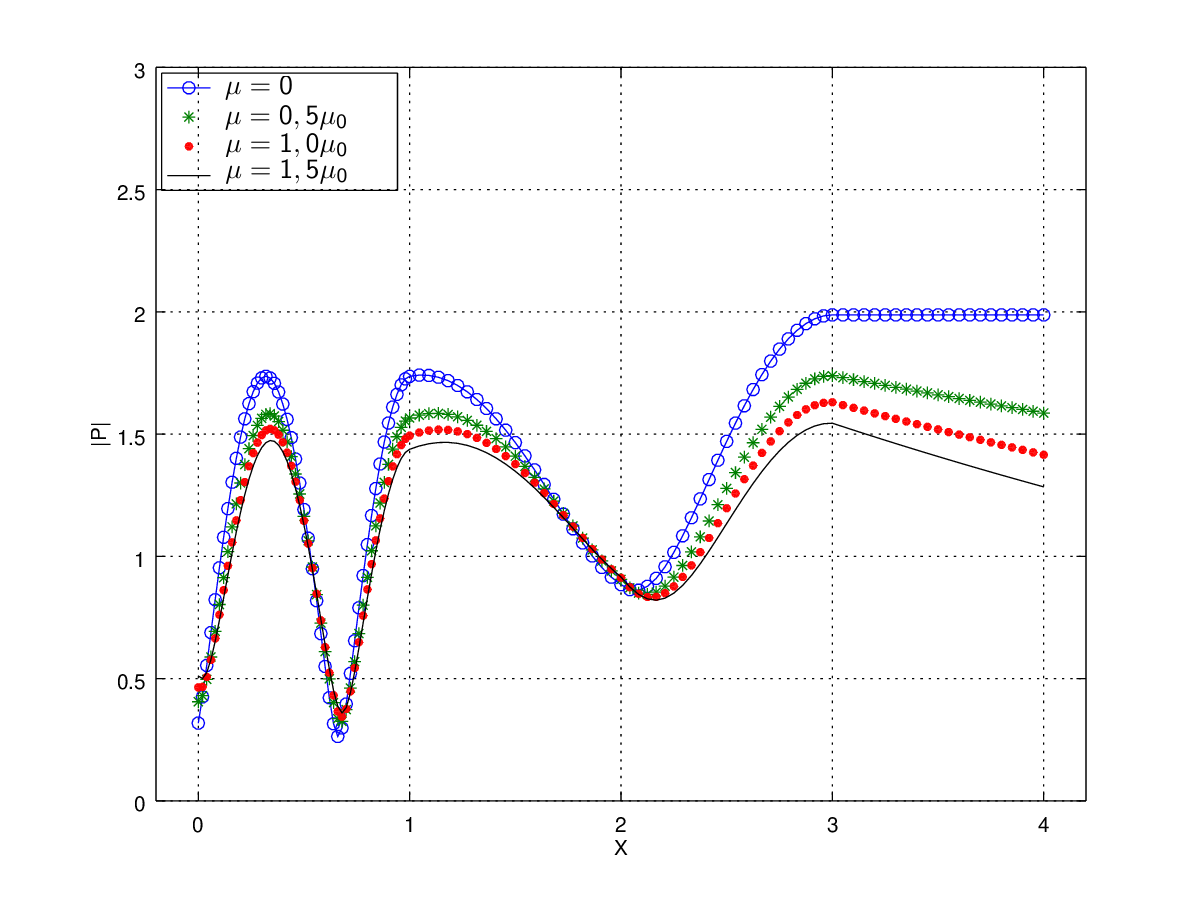
\includegraphics[scale=0.7]{Figures/fig3_P_f14_60_visc_NEW.png}\\
	\caption{Amplitude da pressão $|P|$ ao longo da árvore arterial considerando diferentes viscosidade do fluido $\mu$ e frequências: (a) $f$ = 10,95 Hz, (b)  $f$ = 14,60 Hz. }
	\label{fig3b:arterial-tree}%
\end{figure}

%--------------------------------------------------------------------------------%
\section{SEGMENTO VISCOELÁSTICO}\label{sec:cenario2}

Nas Figuras~\ref{fig4a:arterial-tree}, \ref{fig4b:arterial-tree}, o efeito da viscoelasticidade da parede do segmento de vaso é considerado separadamente considerando-se o escoamento invíscido e tomando-se quatro valores diferentes da viscoelasticidade da parede do segmento. O modelo viscoelástico proposto utilizado para fins destes cálculos é apresentado no cenário 2 da Seção~\ref{sec:cenario}, no qual a viscoelasticidade da parede do vaso é representada por um módulo de Young complexo. Estas figuras mostram os resultados para $\phi_0$ = $0^o$, $4^o$, $8^o$ e $12^o$. Quando $\phi_0$ = $0^o$ tem-se um valor representando uma parede puramente elástica e para $\phi_0> 0$ tem-se a representação da viscoelasticidade. Nota-se a partir destas figuras que o efeito da viscoelasticidade, como o da viscosidade do fluido, é amortecer o aumento global da amplitude da onda de pressão causada pelas reflexões das ondas à medida que a onda se desloca na direção à jusante, bem como moderar os picos locais na distribuição de pressão. 

\begin{figure}[!htbp]
	\centering
	(a) $f$ = 3,65 Hz \\
	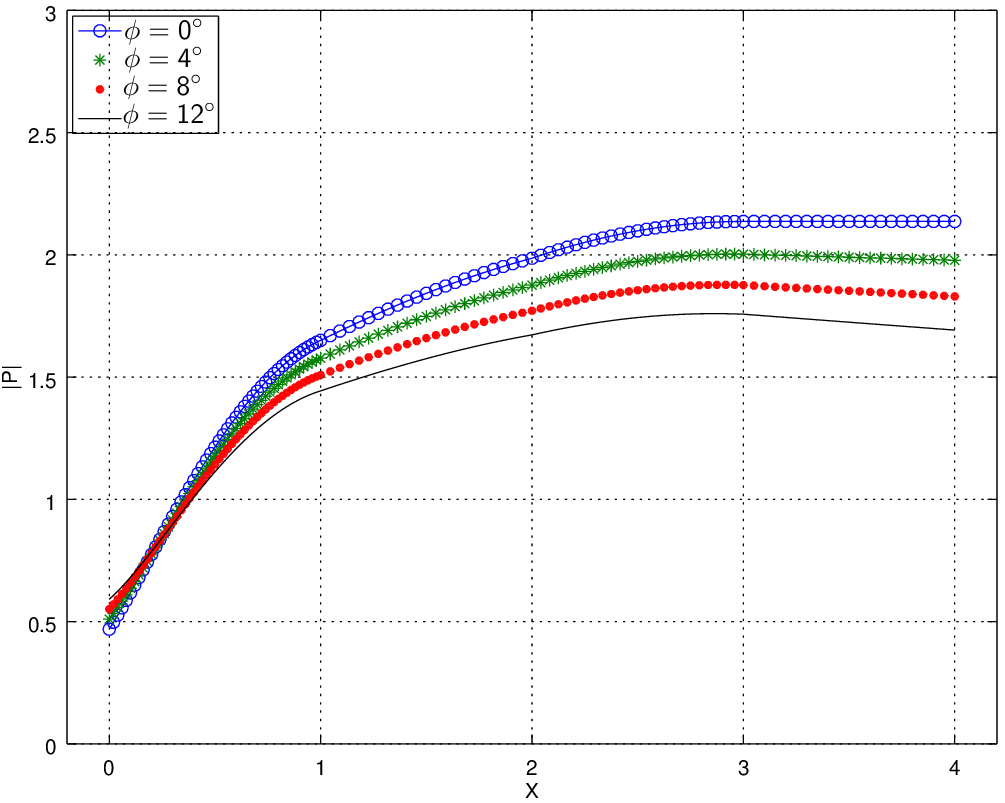
\includegraphics[scale=0.7]{Figures/fig4_P_f3_65_viscoelasticity_NEW.png}\\
	(b)  $f$ = 7,30 Hz\\
	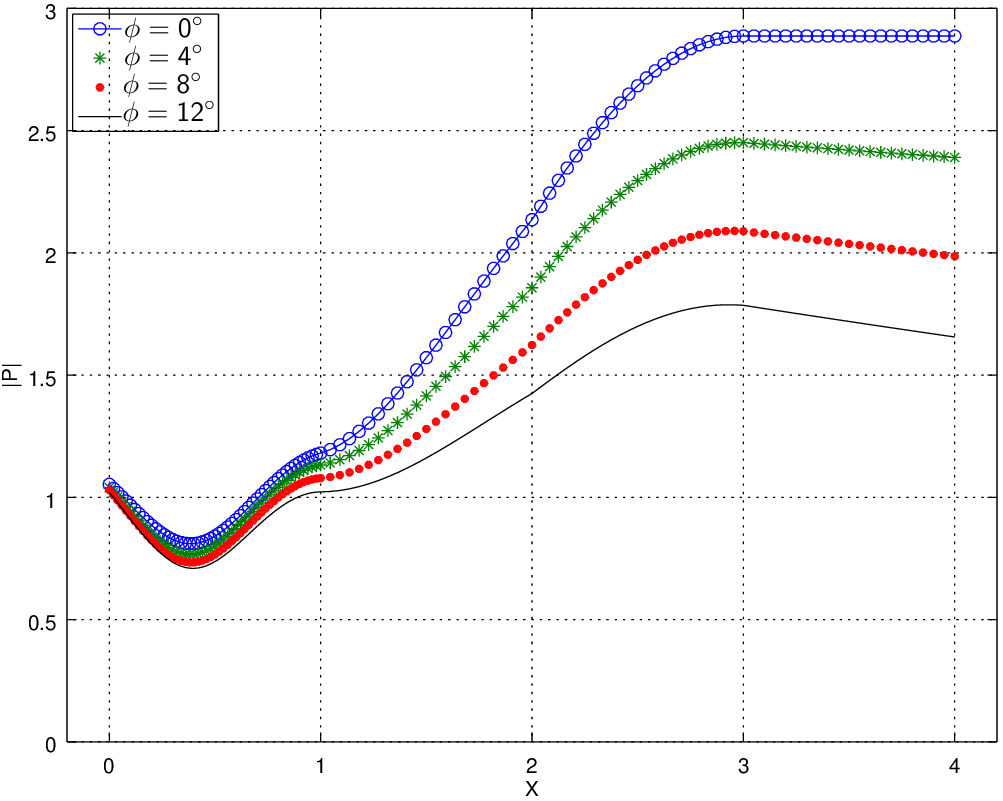
\includegraphics[scale=0.7]{Figures/fig4_P_f7_30_viscoelasticity_NEW.png}\\
	\caption{Amplitude da pressão $|P|$ ao longo da árvore arterial considerando diferentes valores de viscoelasticidade $\phi_0$ e frequências: $f$ = 3,65 Hz e  $f$ = 7,30 Hz. }
	\label{fig4a:arterial-tree}%
\end{figure}

\begin{figure}[!htbp]
	\centering
	(a) $f$ = 10,95 Hz\\
	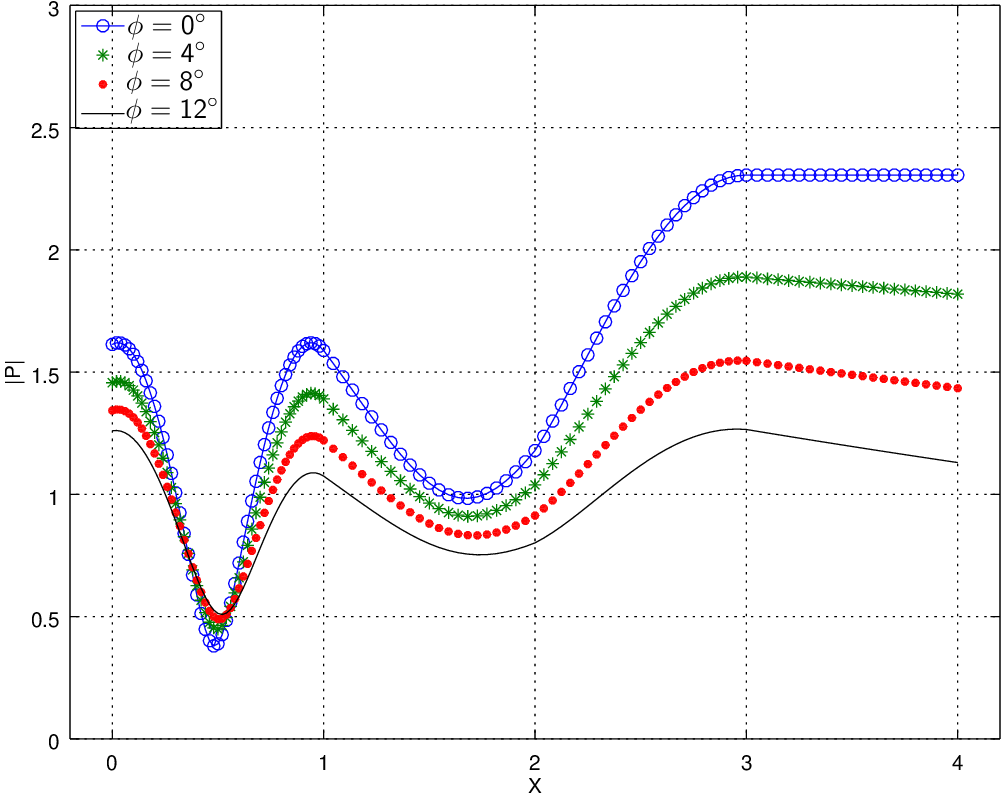
\includegraphics[scale=0.7]{Figures/fig4_P_f10_95_viscoelasticity_NEW.png}\\
	(b) $f$ = 14,60 Hz\\
	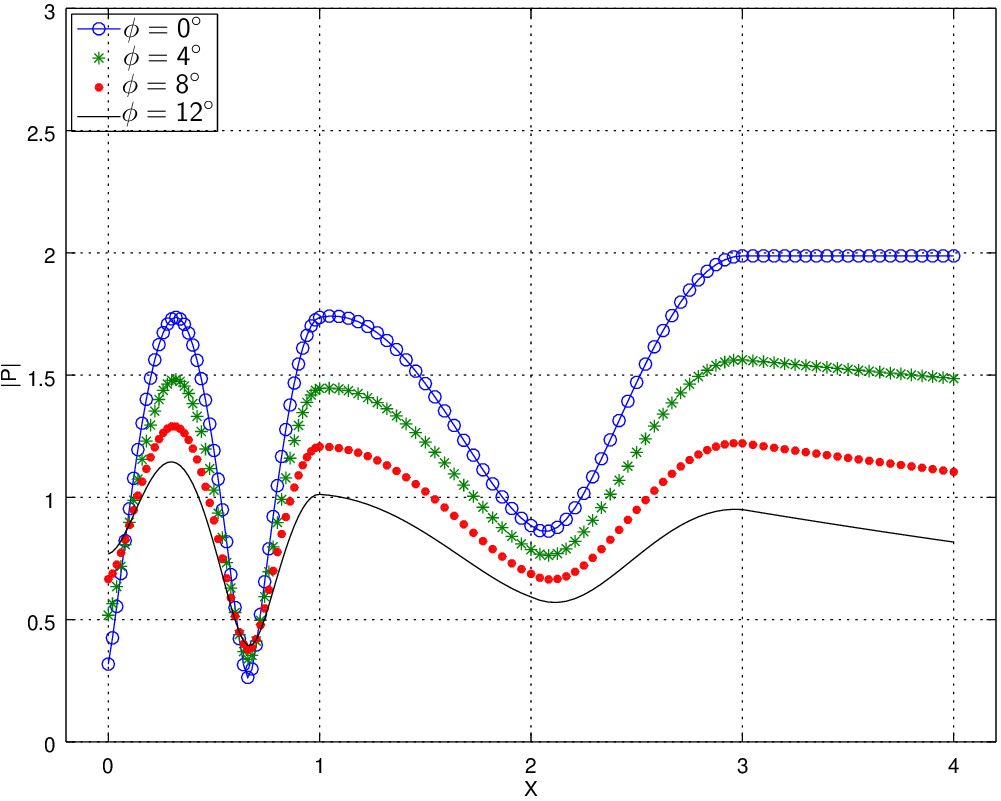
\includegraphics[scale=0.7]{Figures/fig4_P_f14_60_viscoelasticity_NEW.png}\\
	\caption{Amplitude da pressão $|P|$ ao longo da árvore arterial considerando diferentes valores de viscoelasticidade $\phi_0$ e frequências: $f$ = 10,95 Hz e $f$ = 14,60 Hz.}
	\label{fig4b:arterial-tree}%
\end{figure}

%--------------------------------------------------------------------------------%
\section{ESCOAMENTO VISCOSO EM SEGMENTO VISCOELÁSTICO}\label{sec:cenario3}

Nas Figuras~\ref{fig5a:arterial-tree}, \ref{fig5b:arterial-tree}, o efeito da viscoelasticidade da parede do segmento é adicionada ao efeito do escoamento viscoso, adotando dois valores diferentes da viscoelasticidade e dois valores de viscosidade. O modelo utilizado no cenário 3 é a soma dos efeitos apresentados na Seção~\ref{sec:cenario}, adicionando o fator viscoso e o módulo de Young complexo. Estas figuras mostram o resultado para $\phi_0$ = $0^o$, $8^o$ e com as viscosidades $\mu = 0$ e $0,5 \mu_0$. Ao visualizar os efeitos da viscoelasticidade e viscosidade na amplitude da onde de Pressão $P$, é observado o amortecimento global da amplitude de onda de pressão, somado à moderação dos picos locais na distribuição de pressão. Entretanto, o efeito somado dos fenômenos causa um amortecimento mais eficaz que o visto nos outros cenários.

\begin{figure}[!htbp]
	\centering
	(a) \\
	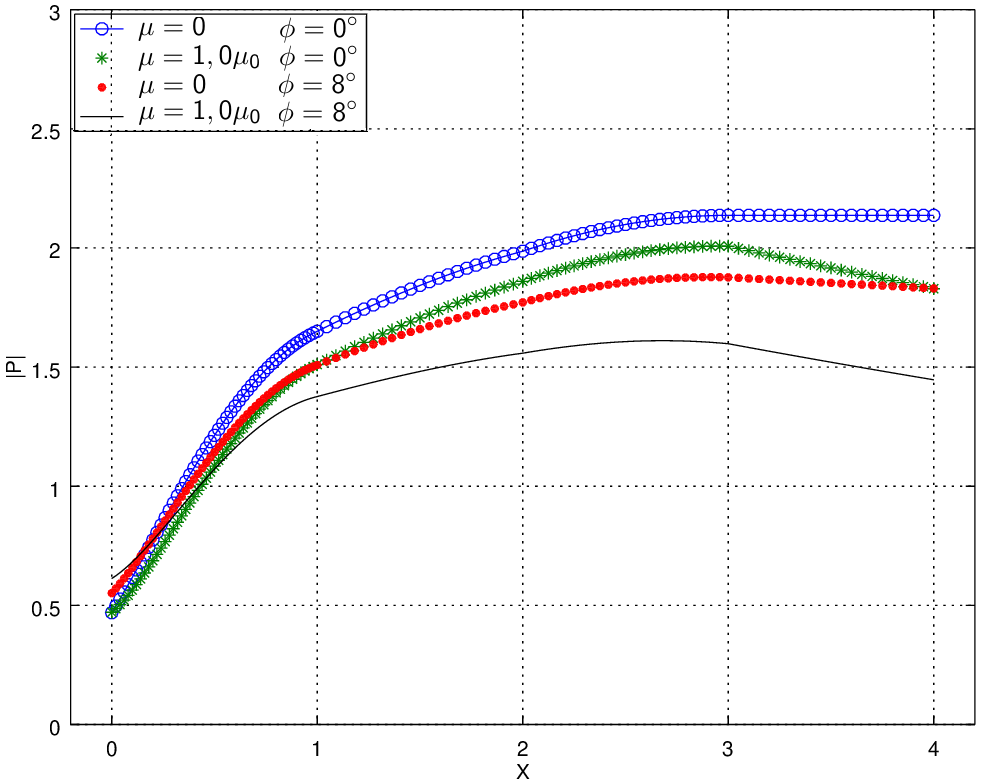
\includegraphics[scale=0.7]{Figures/fig5_P_f3_65_viscoelasticity_viscosity_NEW.png}\\
	(b)\\
	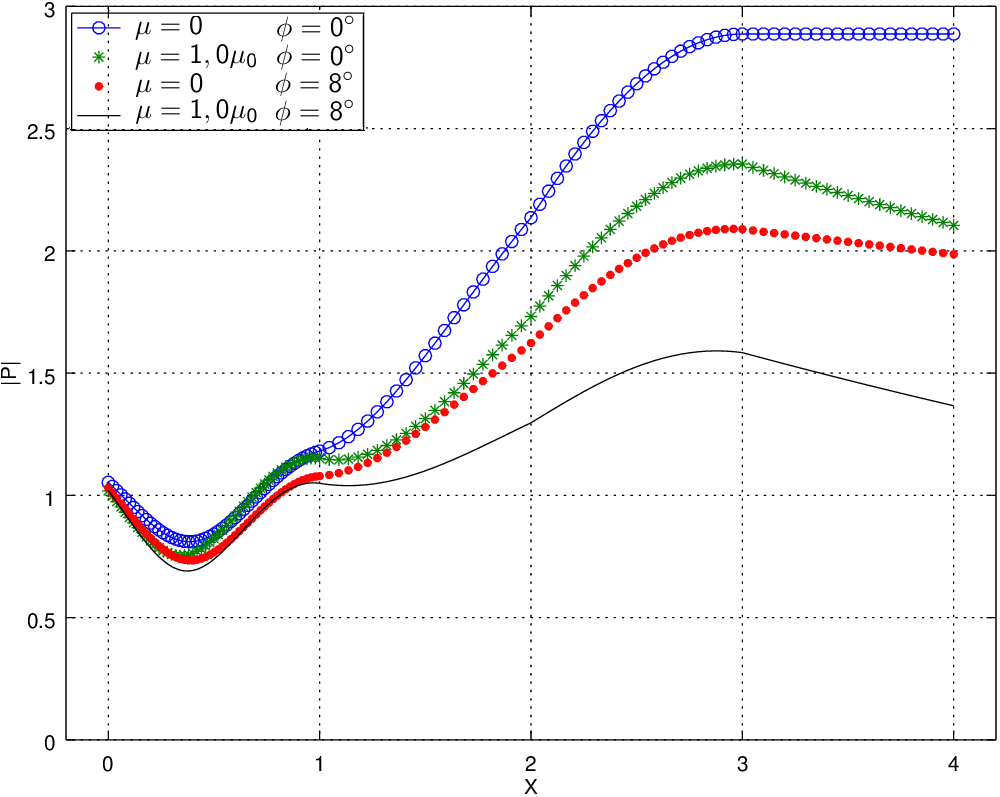
\includegraphics[scale=0.7]{Figures/fig5_P_f7_30_viscoelasticity_viscosity_NEW.png}\\
	\caption{Amplitude da pressão $|P|$ ao longo da árvore arterial considerando diferentes valores de viscoelasticidade $\phi_0$ e frequências: (a) $f$ = 3,65 Hz, (b)  $f$ = 7,30 Hz. }
	\label{fig5a:arterial-tree}%
\end{figure}

\begin{figure}[!htbp]
	\centering
	(a) $f$ = 10,95 Hz\\
	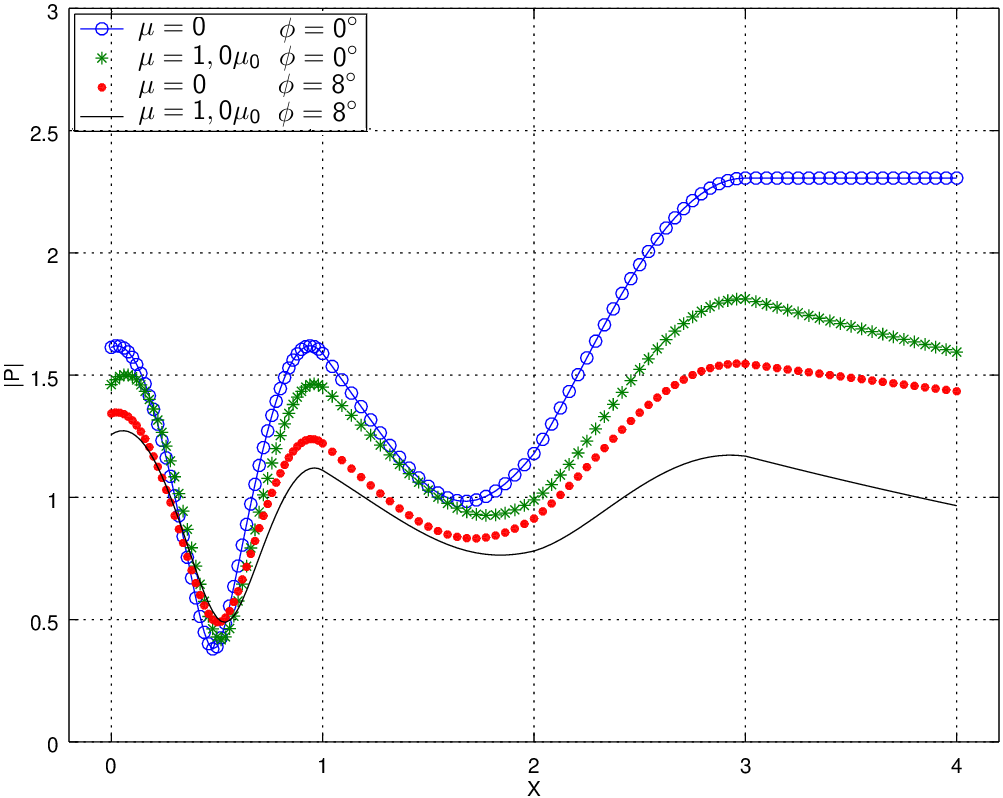
\includegraphics[scale=0.7]{Figures/fig5_P_f10_95_viscoelasticity_viscosity_NEW.png}\\
	(b) $f$ = 14,60 Hz\\
	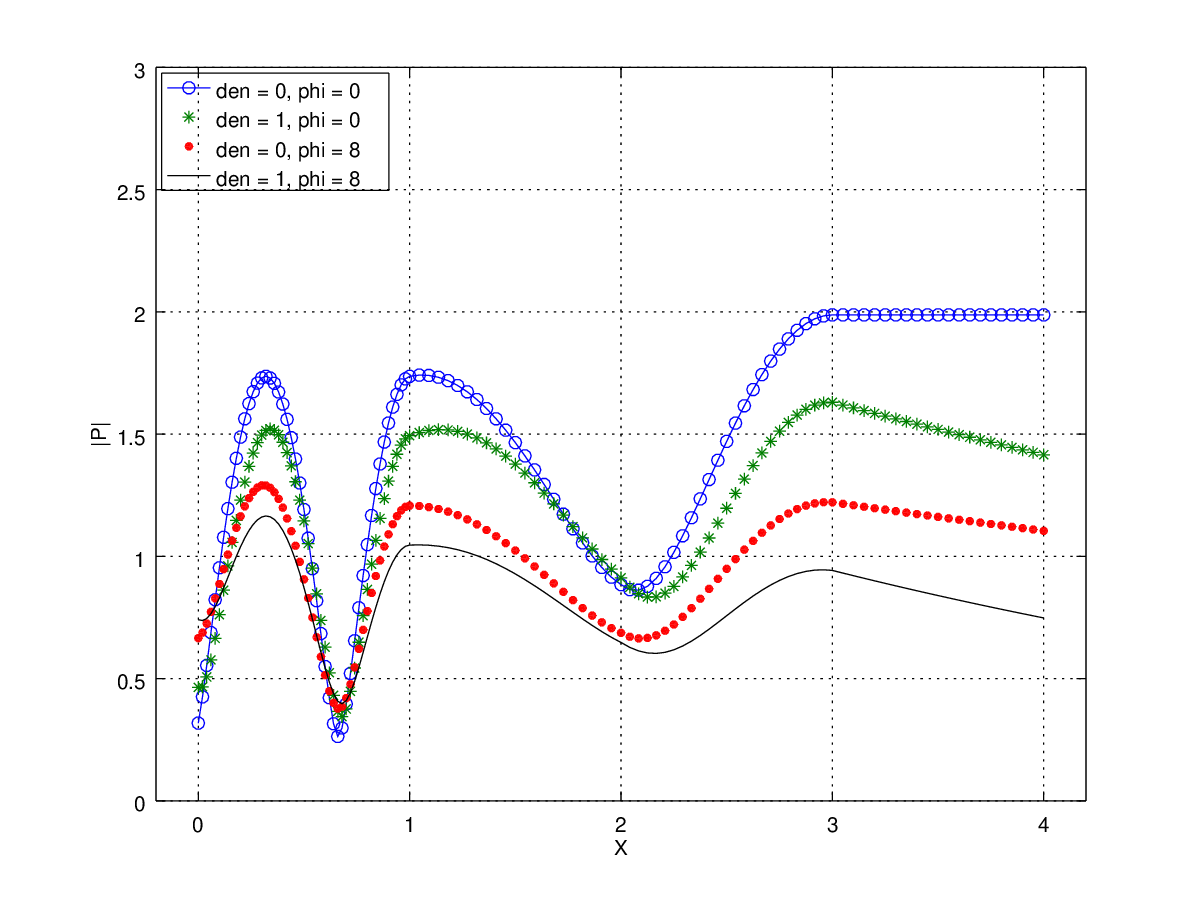
\includegraphics[scale=0.7]{Figures/fig5_P_f14_60_viscoelasticity_viscosity.png}\\
	\caption{Amplitude da pressão $|P|$ ao longo da árvore arterial considerando diferentes valores de viscoelasticidade $\phi_0$ e frequências: (a) $f$ = 10,95 Hz, (b) $f$ = 14,60 Hz.}
	\label{fig5b:arterial-tree}%
\end{figure}

%--------------------------------------------------------------------------------%
\chapter{RESULTADOS COMPUTACIONAIS}\label{sec:resultados2}

Nesta seção, apresentam-se resultados obtidos com a implementação da ferramenta computacional em seus dois ambientes \textit{IGU} e \textit{InGU}. As simulações realizadas aqui tratam da aplicação da ferramenta na obtenção de resultados do escoamento pulsátil em um modelo de árvore arterial. Os resultados de ambas as versões serão apresentados e comparados com a versão anteriormente apresentada.

O arquivo \textit{CMakeList.cmake} é o responsável por interpretar o projeto \textit{Qt} e corretamente compilar as bibliotecas necessárias. Na interface \textit{IDE} do \textit{QtCreator} este arquivo contém as instruções para compilar todos os ambientes e a versão anterior da ferramenta computacional. A versão anterior da ferramenta computacional \textit{IGU} exporta seus resultados em arquivos \textit{VTK}, estes arquivos podem ser lidos pela nova versão ou ainda utilizados em outro ambiente.

Na Figura X observamos como a interface gráfica do usuário possui duas telas de \textit{Canvas} e diversos botões na janela principal. O funcionamento desta interface é muito similar ao da nova interface, entretanto está muito mais ligada exclusivamente à simulação do escoamento pulsátil. Dois \textit{Canvas} possibilitam a exibição de uma árvore arterial e seu gráfico ao mesmo tempo, entretanto prende estes dois elementos na janela principal. Com o esquema de janelas desenvolvido na nova versão da ferramenta é possível que diversos objetos gráficos sejam exibidos ao mesmo tempo.

Outra grande diferença é que o processo iterativo dos modelos estavam atrelado ao uso dos elementos gráficos, sem a possibilidade de executar uma sequência de comandos de uma só vez. Portanto não é possível utilizar a ferramenta computacional nesta versão precisando seu tempo de execução porque o seu processo de configuração requer interação com a interface de usuário. Através dos comandos disponibilizados na Seção~\ref{sec:console} é possível que objetos inteligentes executem uma bateria de comandos e seu desempenho medido e comparado.

Finalmente como visto na Seção 